\documentclass[11pt,notes=hide,aspectratio=169,mathserif]{beamer}

% PACKAGES
\usepackage{graphics}  % Support for images/figures
\usepackage{graphicx}  % Includes the \resizebox command
\usepackage{tikz}      % For flowcharts
\usetikzlibrary{arrows.meta, positioning} % Libraries for TikZ


\usepackage{url}	   % Includes \urldef and \url commands
\usepackage{natbib}
\usepackage{bibentry}  % Includes the \nobibliography command
\usepackage{verbatim}  %Supports comments
\usepackage{booktabs} %Supports \toprule, \bottomrule, etc in tables
\usepackage{etoolbox}  %Supports toggle commands
\usepackage{datetime}
\usepackage{bm}	%Supports bold math \bm
%the LaTeX standard:
\usepackage{cmbright}
\setbeamerfont{frametitle}{family=\fontfamily{cmbr}\selectfont,size=\Large}
\fontencoding{OT1}\fontfamily{cmbr}\selectfont

% PACKAGES (that should already be included by your LyX document settings)
\usepackage{amsfonts}  % Lots of stuff, including \mathbb 
\usepackage{amsmath}   % Standard math package
\usepackage{amsthm}    % Includes the comment functions
\usepackage{subcaption}

% CUSTOM DEFINITIONS
\def\newblock{} %Get beamer to cooperate with BibTeX
\linespread{1.2}

% IDENTIFYING INFORMATION
\title[class]{ECON 326: Economics of Developing Countries \\ TA Session 6}
\author[vaidehi's class ]{Vaidehi Parameswaran (Northwestern Econ)}
\date{\monthname[\the\month] \the\year}

% THEMATIC OPTIONS
%\setbeamercovered{transparent}
\usetheme{metropolis}
\definecolor{mycolor}{RGB}{48,7,144} 
\setbeamercolor{frametitle}{bg=mycolor, fg=white} % Frame title color
\setbeamercolor{title separator}{fg=mycolor} 
\setbeamercolor{progress bar}{fg=mycolor} 
\beamertemplatenavigationsymbolsempty
\setbeamertemplate{footline}[frame number]{}
\setbeamertemplate{itemize item}{\small\raisebox{1pt}{\textcolor{mycolor}{$\blacktriangleright$}}}
\setbeamertemplate{itemize subitem}{\footnotesize\raisebox{1pt}{\textcolor{mycolor}{$\triangleright$}}}
\setbeamertemplate{itemize subsubitem}{\tiny\raisebox{1pt}{\textcolor{mycolor}{$\triangleright$}}}

% BACKUP SLIDE NUMBERING
\usepackage{appendixnumberbeamer}

\begin{document}

%---------------------------------------------------------------------
\begin{frame}[plain]
\titlepage
\end{frame}
%---------------------------------------------------------------------


%---------------------------------------------------------------------
\begin{frame}{Today's Agenda}

\begin{itemize}
\item \href{https://watermark.silverchair.com/123-3-1251.pdf?token=AQECAHi208BE49Ooan9kkhW_Ercy7Dm3ZL_9Cf3qfKAc485ysgAAA4MwggN_BgkqhkiG9w0BBwagggNwMIIDbAIBADCCA2UGCSqGSIb3DQEHATAeBglghkgBZQMEAS4wEQQM5oexR9-ezy51iFcTAgEQgIIDNvXO_WEQ2i7wsuSyrFh78JdyLp-nxQ69jjhzdxGYP3-y7cWm9HCEibHmZCw5vYxLPyLgMuYsZ4-LxYgQdiYZPK_zSeH6TFw9pInr2mJSOi2imv1wxlVSSWUiMou-Rp-U9FV6oNqdXRreflmIFwZKyFDIuFsoiN7pgwifThvGph3PMUb2qxD0UywfWjgf4rxeRPij6U49H7-Jin22nCEOW8ZTMHrRVtpVNmB4p3bwYwPzBwWfxoBwoQfd67OIvlZTpOD2C2XYpMAYjdPHyagmzHxCCTCLODnDBpEqpDls5XpdX24PJQ7H9PhBkEC4Qpa2DzDKKDZNgITi_otp491HJMc1GwAanJ-Uku_RgpBRy6cR4IG4FRZ3UCHa-Sh34UVVrOAVxZVaTTSMaE4733QHq_BeunEY17lRYOaj2zSgPpsXcvQ2L3X-bHXIIL2Sb5V0J7ZF7dXf0rI3Jl_jnPnSAxoYmVbIkyVRprv8YtB-P157Y3majgNT9RF4Cb3df1knyA1xOmLo02_a62Cl9Ye9murC4pUeU1S91DmM8dhRDO8JcN9qPyk2cekq1zjMm37TDzGEfWuOvaYZEES-jF-CAbUj8NgGULPQNLKm8rlje2vN6dEQJ8tSLncpAQHcs7qUqEyio0rnt_njur48ztBQkz8-7BowOICkn7jxg9PiVH03YrtkfezXh_WmvnB4zts9YUNcRIKpel0Z55OqPbUyr4iiXSdPTrS91JSzxMAwst5Antpju-nVDy4EGF9QITvHxsZH-VVpLRoxxQi8bdZHc_lIf6oxxMStsVnoeVX49L0EF_g5I1pazvMcPWNrjlfXGnvqELG9NvvBTHd00DGx9VK67F9T18soSQgJ8Mo1LNL8w20Ok_wY9EvFfDuYJ1GxGNPPN0u-pY-J2YFi9GI00KJ5mF6MDtkMCpikpf4zMhGdatHzfgJZO_DSxh3PMmEtQvvyfPWRfcMh7qxiOJbvuk614KWUsVNP1L7_DfQeeuN_4kOe8DdJ0DUtbsAsAtaR62L78jxemb0Ya1iLrUUbN7D9jwackNp4wZPFTfaC1_qXyHOgURoMQ_eUdI18Q1l1IGnhrZ4ZGQ}{\textcolor{blue}{Qian (2008)}}
\item Midterm Exam
\end{itemize}
\end{frame}
%---------------------------------------------------------------------



\section*{\href{https://watermark.silverchair.com/123-3-1251.pdf?token=AQECAHi208BE49Ooan9kkhW_Ercy7Dm3ZL_9Cf3qfKAc485ysgAAA4MwggN_BgkqhkiG9w0BBwagggNwMIIDbAIBADCCA2UGCSqGSIb3DQEHATAeBglghkgBZQMEAS4wEQQM5oexR9-ezy51iFcTAgEQgIIDNvXO_WEQ2i7wsuSyrFh78JdyLp-nxQ69jjhzdxGYP3-y7cWm9HCEibHmZCw5vYxLPyLgMuYsZ4-LxYgQdiYZPK_zSeH6TFw9pInr2mJSOi2imv1wxlVSSWUiMou-Rp-U9FV6oNqdXRreflmIFwZKyFDIuFsoiN7pgwifThvGph3PMUb2qxD0UywfWjgf4rxeRPij6U49H7-Jin22nCEOW8ZTMHrRVtpVNmB4p3bwYwPzBwWfxoBwoQfd67OIvlZTpOD2C2XYpMAYjdPHyagmzHxCCTCLODnDBpEqpDls5XpdX24PJQ7H9PhBkEC4Qpa2DzDKKDZNgITi_otp491HJMc1GwAanJ-Uku_RgpBRy6cR4IG4FRZ3UCHa-Sh34UVVrOAVxZVaTTSMaE4733QHq_BeunEY17lRYOaj2zSgPpsXcvQ2L3X-bHXIIL2Sb5V0J7ZF7dXf0rI3Jl_jnPnSAxoYmVbIkyVRprv8YtB-P157Y3majgNT9RF4Cb3df1knyA1xOmLo02_a62Cl9Ye9murC4pUeU1S91DmM8dhRDO8JcN9qPyk2cekq1zjMm37TDzGEfWuOvaYZEES-jF-CAbUj8NgGULPQNLKm8rlje2vN6dEQJ8tSLncpAQHcs7qUqEyio0rnt_njur48ztBQkz8-7BowOICkn7jxg9PiVH03YrtkfezXh_WmvnB4zts9YUNcRIKpel0Z55OqPbUyr4iiXSdPTrS91JSzxMAwst5Antpju-nVDy4EGF9QITvHxsZH-VVpLRoxxQi8bdZHc_lIf6oxxMStsVnoeVX49L0EF_g5I1pazvMcPWNrjlfXGnvqELG9NvvBTHd00DGx9VK67F9T18soSQgJ8Mo1LNL8w20Ok_wY9EvFfDuYJ1GxGNPPN0u-pY-J2YFi9GI00KJ5mF6MDtkMCpikpf4zMhGdatHzfgJZO_DSxh3PMmEtQvvyfPWRfcMh7qxiOJbvuk614KWUsVNP1L7_DfQeeuN_4kOe8DdJ0DUtbsAsAtaR62L78jxemb0Ya1iLrUUbN7D9jwackNp4wZPFTfaC1_qXyHOgURoMQ_eUdI18Q1l1IGnhrZ4ZGQ}{\textcolor{blue}{Qian (2008)}} \\[5mm] 
\textnormal{\small{Missing Women and the Price of Tea in China: The Effect of Sex-Specific Earnings on Sex Imbalance}}}

%---------------------------------------------------------------------
\begin{frame}{Overview}
\begin{itemize}
\item Estimates the effect of sex-specific income on sex-differential survival of children, using exogenous variation in the former
\pause \item Preview of findings:
\begin{itemize}
    \pause \item Increasing female income improves survival rates for girls and educational attainment for all children
    \pause \item Increasing male income worsens survival rates for girls and decreases educational attainment for girls without increasing boys' educational attainment
\end{itemize}
\end{itemize}
\end{frame}
%---------------------------------------------------------------------

%---------------------------------------------------------------------
\begin{frame}{What's the endogeneity issue?}
What's the threat to identification in the cross-section?
\begin{itemize}
\pause \item Omitted variable issue: other reasons may cause women's status to be higher in certain areas, which would affect both women's income share and girls' outcomes
\pause \item Calls for an instrumental variable approach!
\end{itemize}
\end{frame}
%---------------------------------------------------------------------

%---------------------------------------------------------------------
\begin{frame}{Context}
\begin{itemize}
\item Policy change: Post-Mao liberalization of agriculture under the “household responsibility system” led to an increase in the production of cash crops (tea, orchards, vegetables) relative to cereals after 1979
\pause \item Two main reforms:
\begin{itemize}
    \pause \item Devolved responsibilities to households
    \pause \item Increased procurement prices
\end{itemize}
\pause \item Differential impact on sex-specific income: Tea is a crop where women have a comparative advantage, whereas orchard is a crop where men have a comparative advantage
\end{itemize}
\end{frame}
%---------------------------------------------------------------------

%---------------------------------------------------------------------
\begin{frame}{Variation over time induced by policy change}
\begin{figure}
\centering
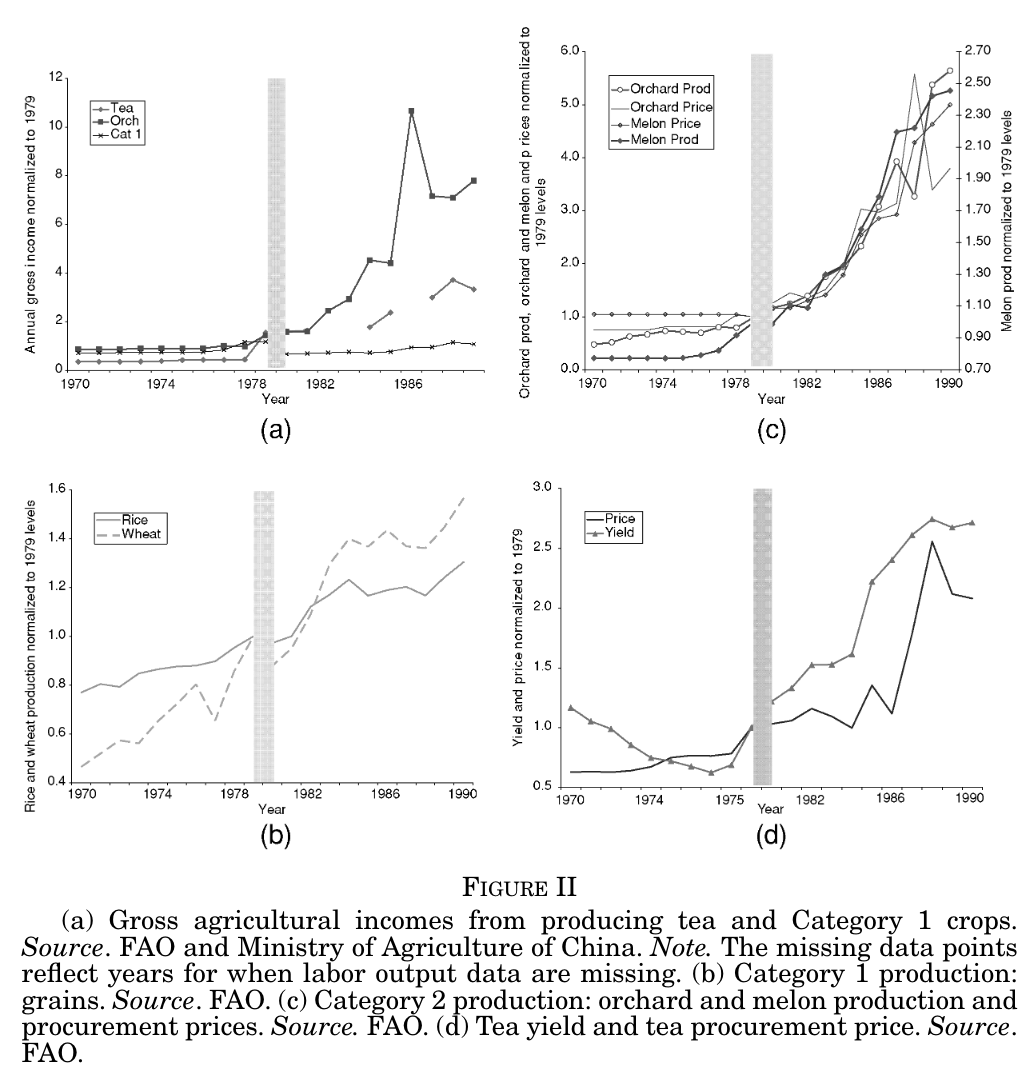
\includegraphics[width=0.5\textwidth]{inputs/fig2.png}
\end{figure}
\end{frame}
%---------------------------------------------------------------------

%---------------------------------------------------------------------
\begin{frame}{Diff-in-diff Plot}
\begin{itemize}
\item Suppose parents respond to expected returns of having boys and girls
\pause \item What would you expect to see if you plotted the gender ratio over time in regions suitable to tea production vs. other regions?
\end{itemize}
\pause 
\begin{figure}
\centering
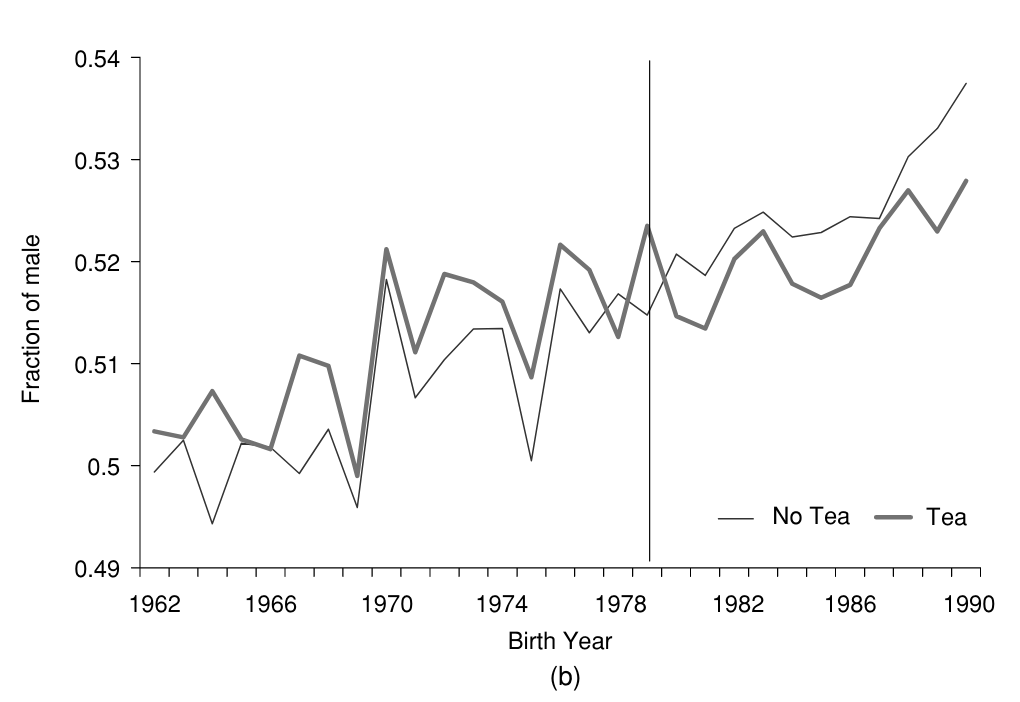
\includegraphics[width=0.58\textwidth]{inputs/fig3b.png}
\end{figure}
\end{frame}
%---------------------------------------------------------------------

%---------------------------------------------------------------------
\begin{frame}{Diff-in-diff Strategy}
\begin{itemize}
\item Compare sex ratio:
\begin{itemize}
    \pause \item Before and after the reform:  Comparing within counties across cohorts differences out time-invariant community characteristics
    \pause \item Tea producing and non tea producing regions: Comparing within cohorts between tea-planting and non-tea-planting communities differences out changes over time that affect these regions similarly
\end{itemize}
\pause \item Then difference the differences 
\item Estimating equation:
\pause \begin{align*}
s_{ik} = \alpha + \beta POST + \delta TEA + \gamma (POST \times TEA) + \epsilon_{ik}
\end{align*}
, where $\gamma$ is the difference-in-difference estimate of the effect of growing tea on sex ratios
\end{itemize}
\end{frame}
%---------------------------------------------------------------------

%---------------------------------------------------------------------
\begin{frame}{Identification}
\begin{itemize}
\item Parallel trends assumption
\begin{itemize}
    \pause \item No change in sex preferences in tea counties during the same time as the reform
    \pause \item No other changes in tea counties during the same time of the reform
\end{itemize}
\pause \item The decision to plant tea not affected by sex preference. Why
does she need this assumption?
\end{itemize}
\end{frame}
%---------------------------------------------------------------------

%---------------------------------------------------------------------
\begin{frame}{Basic diff-in-diff results}
\begin{figure}
\centering
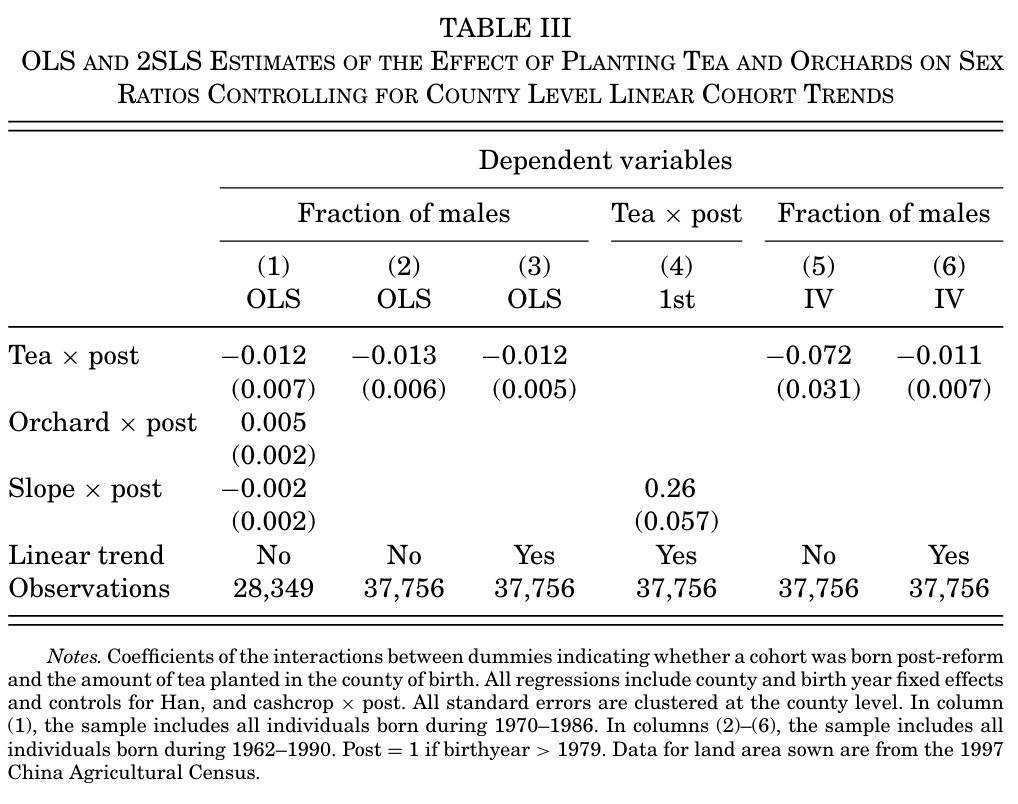
\includegraphics[width=0.5\textwidth]{inputs/table3.png}
\end{figure}
\end{frame}
%---------------------------------------------------------------------

%---------------------------------------------------------------------
\begin{frame}{Generalise in two steps}
\begin{itemize}
\item Step 1: Include one dummy per cohort, and one dummy per county
\begin{align*}
s_{ik} = \alpha + \sum_t \beta_t D_t + \sum_j \delta_j D_j + \gamma (POST_k \times TEA_i) + \epsilon_{ik}
\end{align*}
where $D_k = 1$ if $t = k$ and $0$ otherwise, $D_j =1$ if $i = j$ and $0$ otherwise
\item Step 2:  Include an interaction per cohort
\begin{align*}
s_{ik} = \alpha + \sum_t \beta_t D_t + \sum_j \delta_j D_j + \sum_t \gamma_t (D_t \times TEA_i) + \epsilon_{ik}
\end{align*}
\end{itemize}
\end{frame}
%---------------------------------------------------------------------

%---------------------------------------------------------------------
\begin{frame}{Plot the $\gamma_k$}
\begin{figure}
\centering
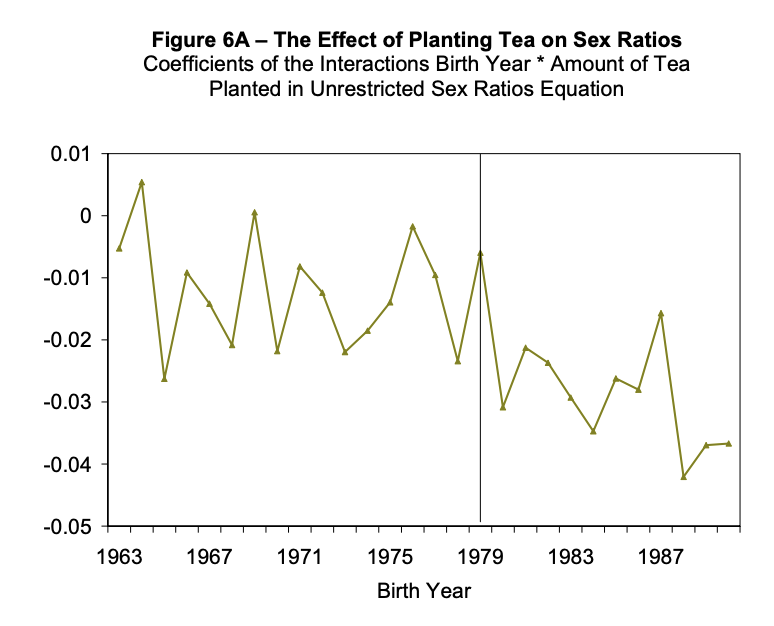
\includegraphics[width=0.5\textwidth]{inputs/tea.png}
\end{figure}
\end{frame}
%---------------------------------------------------------------------

%---------------------------------------------------------------------
\begin{frame}{Introducing orchards as control group}
\begin{itemize}
\item What if the effect is not about tea, but about cash crops in general?
\pause  \item What would you expect to see if you plotted the gender ratio over time in regions suitable to orchard production and in other regions?
If you repeated the diff-in-diff analysis but with orchards?
\pause  \begin{align*}
s_{ik} = \alpha + \sum_t \beta_t D_t + \sum_j \delta_j D_j + \lambda_t (D_t \times ORCHARD_i) + \epsilon_{ik}
\end{align*}
\end{itemize}
\end{frame}
%---------------------------------------------------------------------

%---------------------------------------------------------------------
\begin{frame}{Orchards}
\begin{figure}
\centering
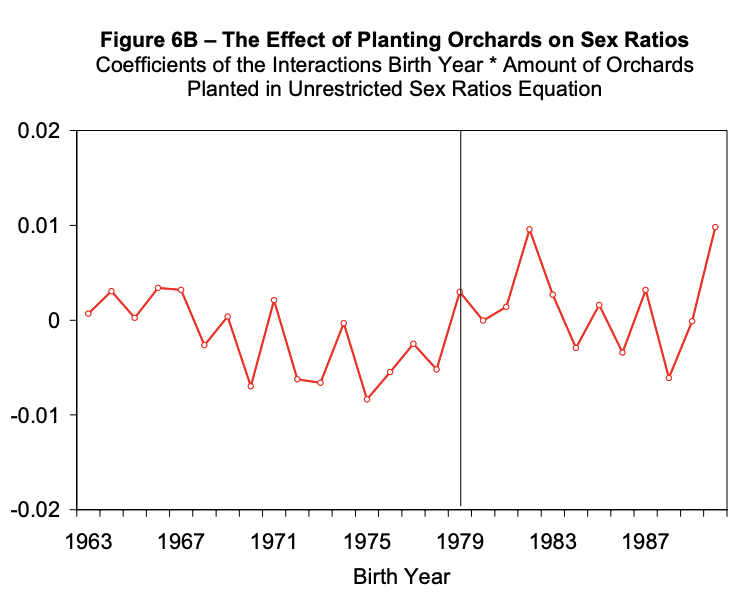
\includegraphics[width=0.5\textwidth]{inputs/orchards.png}
\end{figure}
\end{frame}
%---------------------------------------------------------------------

%---------------------------------------------------------------------
\begin{frame}{Placebo test}
\begin{figure}
\centering
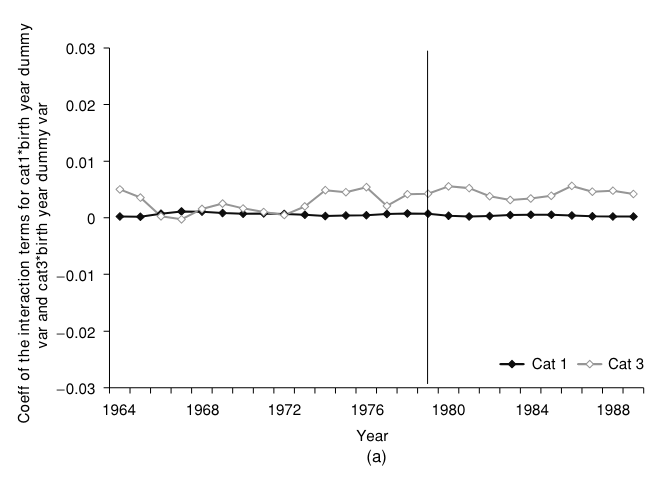
\includegraphics[width=0.5\textwidth]{inputs/fig3a.png}
\end{figure}
\begin{itemize}
    \pause  \item Category 1: grains, that did not become unregulated
    \pause  \item Category 3:  vegetable patches that had never been regulated
\end{itemize}
\end{frame}
%---------------------------------------------------------------------

%---------------------------------------------------------------------
\begin{frame}{Test of income effect}
\begin{figure}
\centering
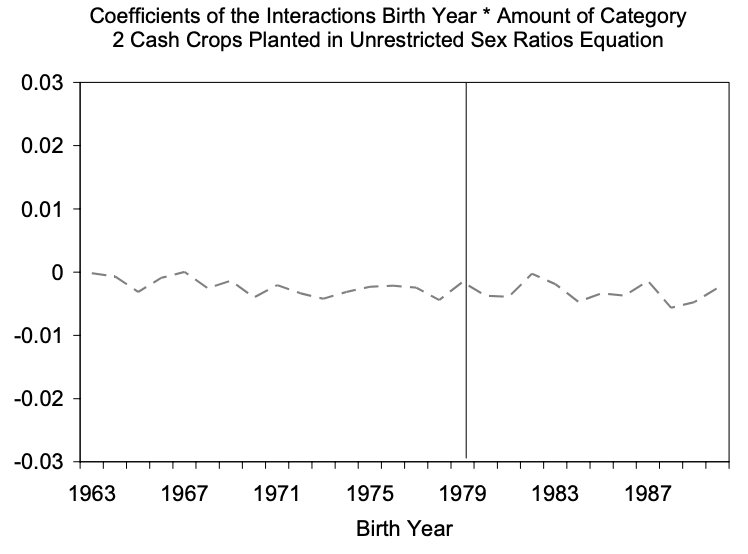
\includegraphics[width=0.5\textwidth]{inputs/inc.png}
\end{figure}
\begin{itemize}
\item All cash crops taken together have no effect
\end{itemize}
\end{frame}
%---------------------------------------------------------------------

%---------------------------------------------------------------------
\begin{frame}{Introducing orchards and tea together in one regression}
\begin{itemize}
\item For precise estimation, in the paper all the data are pooled together in one big regression with three sets of dummies
\begin{align*}
    s_{ik} = \alpha + \beta POST_k + \sum_j \delta_j D_j +  \gamma_t (D_t \times TEA_i) + \sum_t \lambda_t (D_t \times ORCHARD_i) + \epsilon_{ik}
\end{align*}
\end{itemize}
\end{frame}
%---------------------------------------------------------------------

%---------------------------------------------------------------------
\begin{frame}{Yearly coefficients}
\begin{figure}
\centering
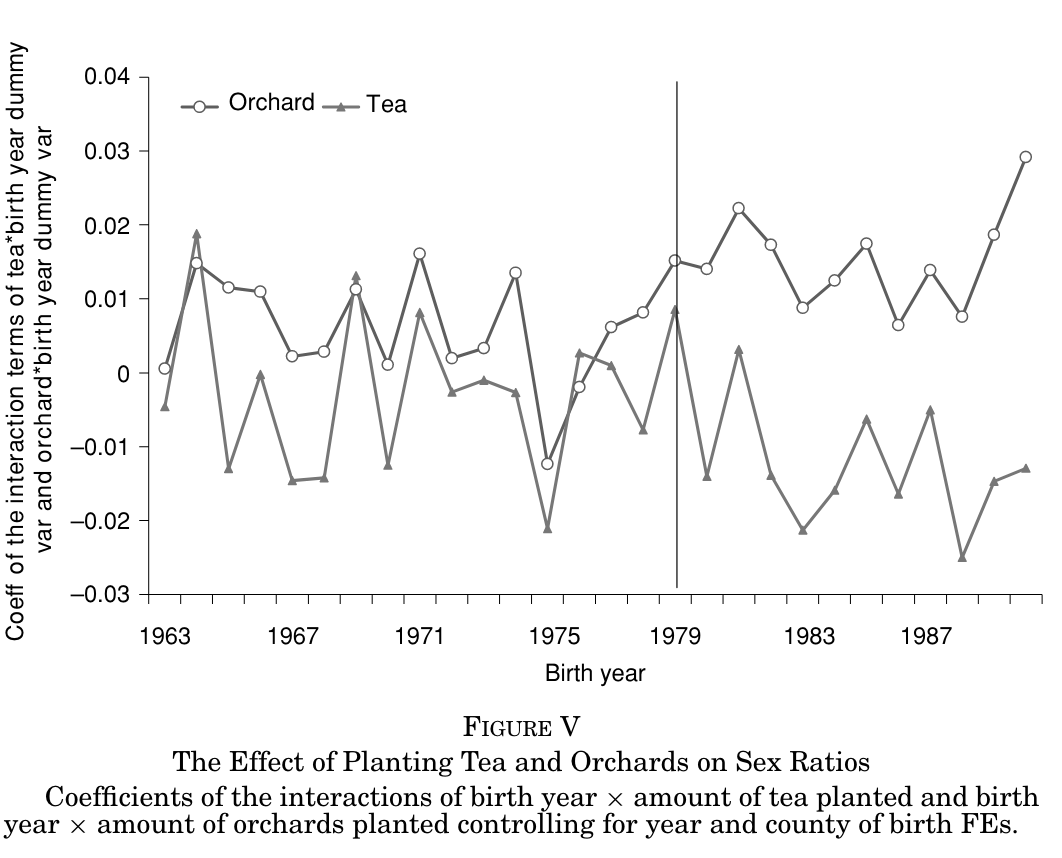
\includegraphics[width=0.5\textwidth]{inputs/fig5.png}
\end{figure}
\end{frame}
%---------------------------------------------------------------------

%---------------------------------------------------------------------
\begin{frame}{Differential effect on girls' education}
Same regression but with education as the dependent variable
\begin{figure}
\centering
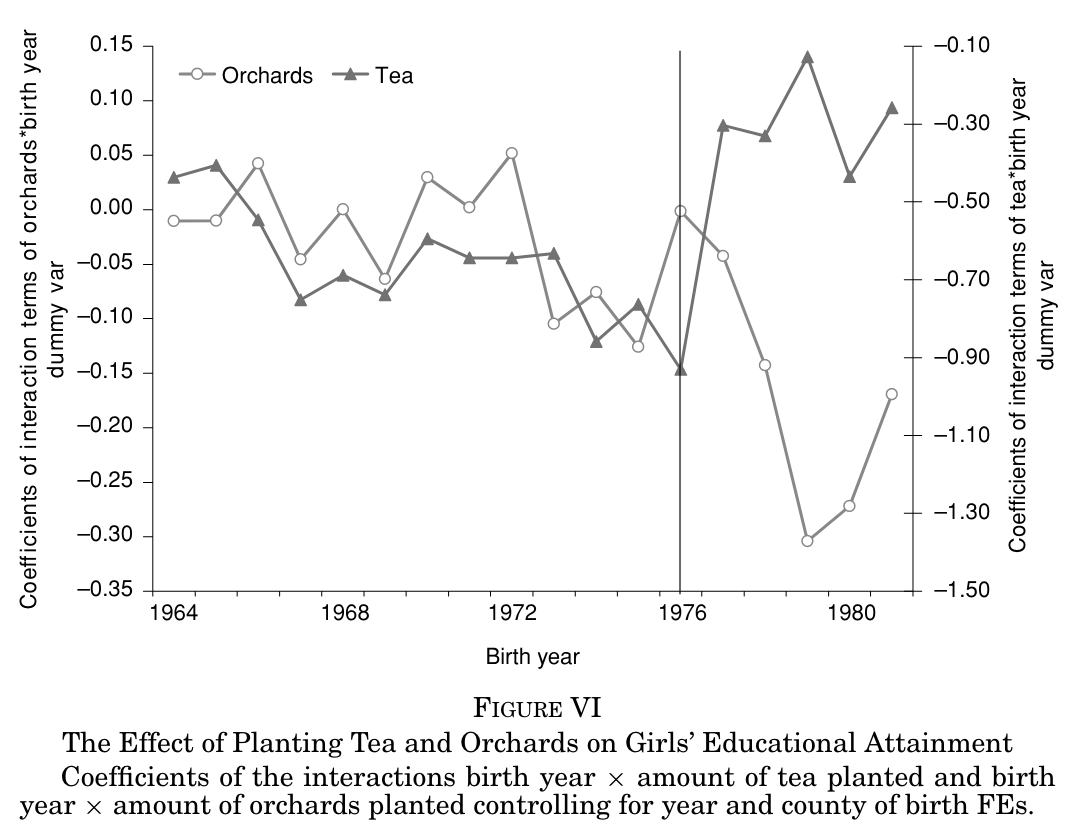
\includegraphics[width=0.5\textwidth]{inputs/fig6.png}
\end{figure}
\end{frame}
%---------------------------------------------------------------------

%---------------------------------------------------------------------
\begin{frame}{Dicussion and interpretation}
\begin{itemize}
\item What if people who like girls grow tea? What is a potential strategy to deal with it?
\pause \item Instrument for tea production using suitability of land for tea production (hilliness / slope of land)
\pause \item Common use case of instruments: providing exogenous variation for a variable which we worry is endogenous
\end{itemize}
\begin{figure}
\centering
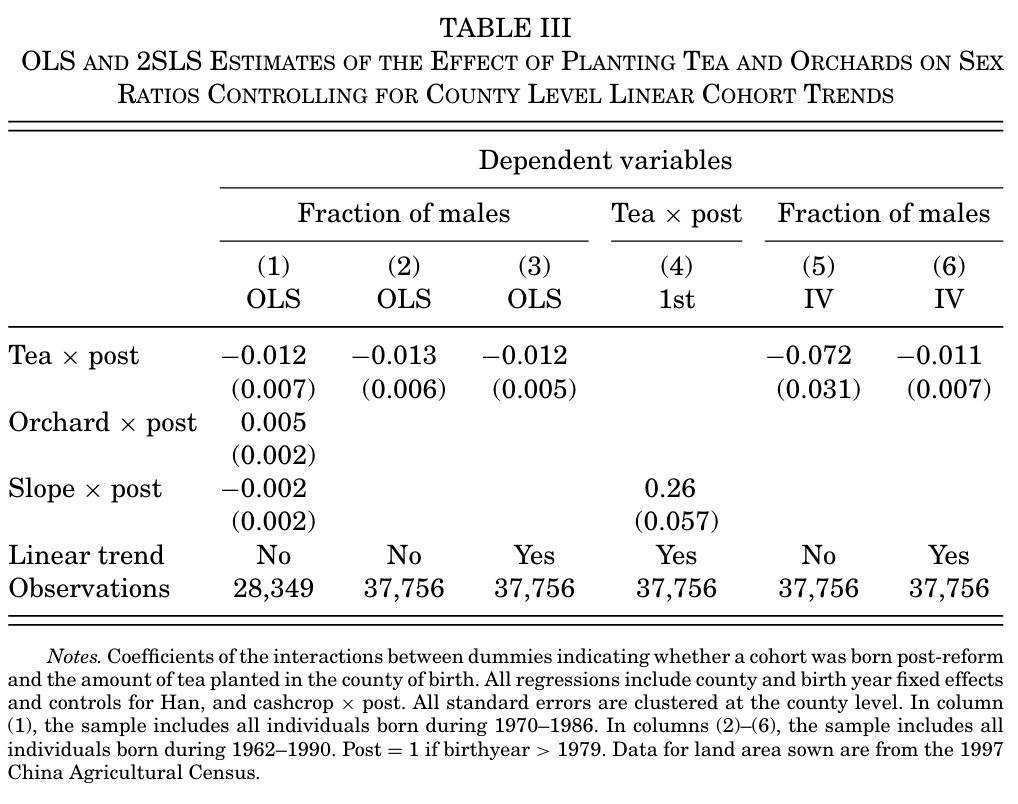
\includegraphics[width=0.4\textwidth]{inputs/table3.png}
\end{figure}
\end{frame}
%---------------------------------------------------------------------

%---------------------------------------------------------------------
\begin{frame}{Mechanisms}
\begin{itemize}
\item Are we sure it is about higher returns to girls?
\pause \item What else does an increase in womens’ relative wages cause, immediately?
\end{itemize}
\end{frame}
%---------------------------------------------------------------------

\section*{Midterm Exam}

%---------------------------------------------------------------------
\begin{frame}
\begin{center}{\LARGE See you next time!}\end{center}
\end{frame}
%---------------------------------------------------------------------


\end{document}
